% #############################################################################
% This is Chapter 6
% !TEX root = ../main.tex
% #############################################################################
\fancychapter{Results}
% The following line allows to ref this chapter
\label{chap:results}

This chapter answers the four research questions: what the applications look like (RQ1, Section~\ref{sec:res-rq1}), what data reaches their AI components (RQ2, Section~\ref{sec:res-rq2}), how prevalent the preconditions for attacks are (RQ3, Section~\ref{sec:res-rq3}), and how reliable these measurements are (RQ4, Section~\ref{sec:res-rq4}). Results are reported per repository, relative to the repositories in which each property can occur, and use the confirmed rules of Chapter~\ref{sec:toolkit} unless marked as an upper bound.

\paragraph{Coverage.} Of the 381 repositories selected for the data-flow analysis, 379 were analysed; the remaining two no longer exist on GitHub (Table~\ref{tab:dataflow-coverage}). 304 of the analysed repositories contain at least one AI sink (313 including heuristic detections). Test files located next to the source code are excluded from all results (Section~\ref{sec:df-limitations}); including them changes each risk pattern by at most one repository, but inflates the share of static inputs, because test fixtures pass fixed prompts and documents to the applications' AI components.

% =============================================================================
\section{RQ1: What Do Agentic Applications Look Like?}
\label{sec:res-rq1}

Framework usage in RADAR is led by the OpenAI SDK ($65.9\%$ of applications) and the MCP SDK ($57.4\%$) (Figure~\ref{fig:framework-summary}), and the applications span 15 domains, led by developer tools and coding agents (154) and general-purpose agent platforms (122) (Table~\ref{tab:topic-counts}). The corpus is thus dominated by applications that call models directly through a vendor SDK and increasingly expose or consume tools through MCP, rather than by applications built on a single orchestration framework.

The data-flow analysis shows which AI components these applications contain. Of the 379 analysed applications, 256 (67.5\%) pass data to a model or agent, 165 (43.5\%) define tools that a model can call, and 59 (15.6\%) use a vector store or agent memory. In 93 applications the output of one model call is the input of another, as in agent pipelines and multi-agent designs.

\emph{Meaning:} a typical application in the corpus is a model-calling application with tools; retrieval and memory are present in a minority, and chained or multi-agent designs in about a quarter of the applications.

% =============================================================================
\section{RQ2: What Data Reaches the AI Components?}
\label{sec:res-rq2}

Across the 379 analysed repositories, the analysis found 24{,}473 sink sites with 32{,}759 input values under the confirmed rules (Table~\ref{tab:res-totals}), and 261{,}575 occurrences of configuration, user, external, and database sources, of which 10{,}852 lie in AI-relevant code. Tool parameters and tool results account for 81\% of the sink values, because a few repositories define hundreds of tools; results are therefore reported per repository. Most source occurrences belong to parts of the applications unrelated to AI, which is why reach is reported for AI-relevant code (Table~\ref{tab:res-reach}).

\begin{table}[t]
\centering
\footnotesize
\renewcommand{\arraystretch}{1.15}
\caption{Totals over the 379 analysed repositories (confirmed rules, test files excluded). A \emph{site} is a code location with a sink; a \emph{value} is one input of a sink, so a site can contribute several values.}
\label{tab:res-totals}
\begin{tabular}{@{}llrr@{}}
\toprule
\multicolumn{4}{@{}l}{\emph{Sinks}} \\
\textbf{Category} & \textbf{Type} & \textbf{Sites} & \textbf{Values} \\
\midrule
model & call         & 3{,}405  & 4{,}422 \\
      & instructions & 702      & 847 \\
      & history      & 100      & 101 \\
tool  & params       & 5{,}393  & 12{,}372 \\
      & effect       & 245      & 252 \\
      & result       & 14{,}291 & 14{,}302 \\
      & dispatch     & 24       & 56 \\
store & write        & 141      & 208 \\
      & query        & 172      & 199 \\
\midrule
\multicolumn{2}{@{}l}{\textbf{Total, confirmed}}          & \textbf{24{,}473} & \textbf{32{,}759} \\
\multicolumn{2}{@{}l}{Additional heuristic values}         &                   & 586 \\
\addlinespace[4pt]
\multicolumn{4}{@{}l}{\emph{Sources}} \\
\textbf{Source} & & \textbf{Occurrences} & \textbf{In AI-relevant code} \\
\midrule
\texttt{config}      & & 66{,}849 & 4{,}086 \\
\texttt{user}        & & 72{,}421 & 2{,}114 \\
\texttt{external}    & & 57{,}305 & 2{,}184 \\
\texttt{database}    & & 65{,}000 & 2{,}468 \\
\midrule
\multicolumn{2}{@{}l}{\textbf{Total, primary sources}}    & \textbf{261{,}575} & \textbf{10{,}852} \\
\addlinespace[2pt]
\texttt{model} (model-call sites)                  & & 3{,}405 & --- \\
\texttt{tool\_result} (tools with a return value)  & & 3{,}470 & --- \\
\texttt{store\_read} (store reads)                 & & 215     & --- \\
\bottomrule
\end{tabular}
\end{table}

\subsection{Which Components Receive Data}

Table~\ref{tab:res-sinks} and Figure~\ref{fig:res-sink-prevalence} give the share of applications containing each sink type. Model calls are the most common (65.4\%), followed by tools: 43.5\% of the applications return tool results to a model and 42.7\% have model-chosen tool parameters, while 13.2\% contain a tool whose model-controlled input reaches a command, file, network, or database operation. Explicit instructions appear in 17.2\%, store writes and queries in 12.9\% and 12.4\%, and hand-written dispatch in only 3.2\%.

\emph{Meaning:} almost half of the applications let the model act through tools, but only about one in seven gives it control over an operation with side effects. Hand-written dispatch is rare because frameworks perform tool dispatch internally.

% \begin{table}[t]
% \centering
% \footnotesize
% \renewcommand{\arraystretch}{1.15}
% \caption{Sinks per type (confirmed rules, test files excluded): applications containing the sink (of 379 analysed), and input classes of its inputs (share of input values).}
% \label{tab:res-sinks}
% \begin{tabular}{@{}llrrrrrr@{}}
% \toprule
% & & \multicolumn{2}{c}{\textbf{Applications}} & \multicolumn{4}{c}{\textbf{Input class (\%)}} \\
% \cmidrule(lr){3-4}\cmidrule(l){5-8}
% \textbf{Category} & \textbf{Type} & \textbf{n} & \textbf{\%} & \textbf{Static} & \textbf{Deploy.} & \textbf{Dynamic} & \textbf{Undet.} \\
% \midrule
% model & call         & 248 & 65.4 & 20.5 & 0.0 & 28.7       & 50.7 \\
%       & instructions & 65  & 17.2 & 80.6 & 0.0 & 3.0        & 16.4 \\
%       & history      & 13  & 3.4  & 5.9  & 1.0 & 54.5       & 38.6 \\
% tool  & params       & 162 & 42.7 & ---  & --- & 100\,$^a$  & --- \\
%       & effect       & 50  & 13.2 & ---  & --- & 100\,$^a$  & --- \\
%       & result       & 165 & 43.5 & 31.0 & 0.1 & 35.5       & 33.4 \\
%       & dispatch     & 12  & 3.2  & 1.8  & 0.0 & 87.5       & 10.7 \\
% store & write        & 49  & 12.9 & 8.7  & 0.0 & 39.9       & 51.4 \\
%       & query        & 47  & 12.4 & 8.5  & 0.0 & 16.6       & 74.9 \\
% \bottomrule
% \multicolumn{8}{@{}l}{\scriptsize $^a$ Model-controlled by definition.}
% \end{tabular}
% \end{table}

\begin{figure}[t]
  \centering
  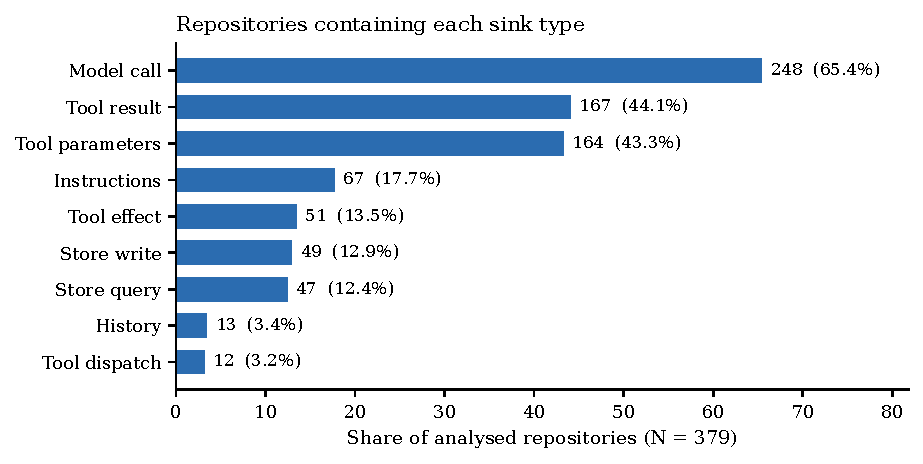
\includegraphics[width=0.85\linewidth]{Images/flow/sink_prevalence.pdf}
  \caption{Share of analysed applications containing each sink type (confirmed rules).}
  \label{fig:res-sink-prevalence}
\end{figure}

\subsection{Fixed or Set at Run Time}

Figure~\ref{fig:res-input-classes} shows the input classes per sink type; tool parameters are excluded because they are model-controlled by definition and far outnumber all other inputs. Instructions are overwhelmingly fixed: 80.6\% of instruction values are static and only 3.0\% are built at run time. Model-call inputs are dynamic in 28.7\%, static in 20.5\%, and undetermined in 50.7\%; store writes are mostly dynamic where their origin is known (39.9\%, against 8.7\% static), and store queries are mostly undetermined (74.9\%).

\emph{Meaning:} developers keep what they \emph{tell} the model under their control; what varies at run time is what the model is \emph{given to read}. The undetermined shares are discussed under RQ4; the dynamic shares are lower bounds.

\begin{figure}[t]
  \centering
  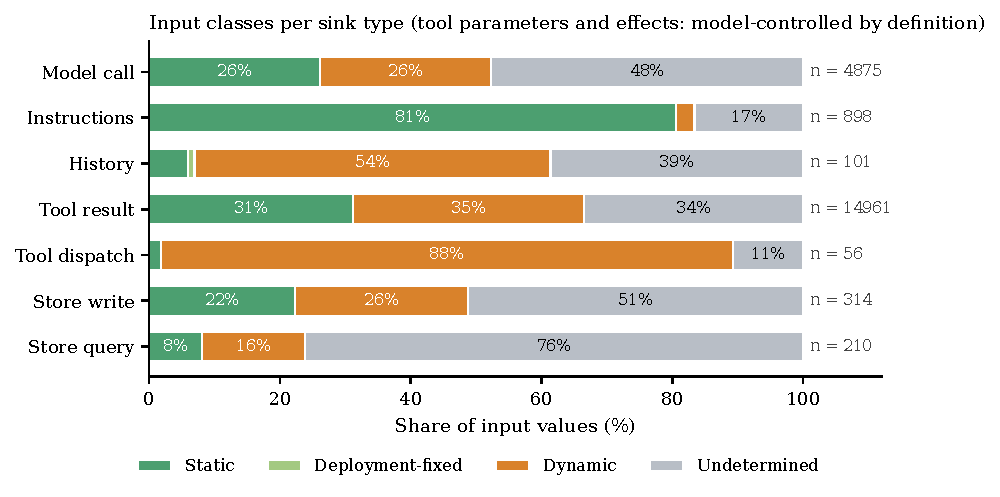
\includegraphics[width=0.85\linewidth]{Images/flow/input_classes.pdf}
  \caption{Input classes per sink type (share of input values, confirmed rules).}
  \label{fig:res-input-classes}
\end{figure}

\subsection{Model Inputs}

Where the message role can be determined, system messages are mostly static (59.3\% of 474 values) but built at run time in 13.5\%; user messages are dynamic in 31.2\% of 478 values. In 93 applications, the output of one model call feeds another model call.

\emph{Meaning:} run-time system messages are where outside content can gain developer-level authority (Section~\ref{sec:res-rq3}); chained model calls mean that content injected into one model can propagate to the next.

\subsection{Tools}

The analysed applications define 3{,}473 tools in 165 applications. Model-controlled input reaches command execution in 18 applications, the file system in 20, network requests in 19, and database operations in 21 (Table~\ref{tab:res-tool-effects}). Tools return external content to the model in 80 applications, database content in 40, and the output of another model call in 127.

\emph{Meaning:} tools play two roles: they bring outside content into the model's context, and in a smaller number of applications they let the model act on the environment. External content enters through tool results in more applications than through any other sink type. Because effects in helper functions are not detected (Section~\ref{sec:df-limitations}), the effect counts are lower bounds.

\begin{table}[t]
\centering
\renewcommand{\arraystretch}{1.2}
\caption{Tool effects whose argument is controlled by the model.}
\label{tab:res-tool-effects}
\begin{tabular}{@{}lrr@{}}
\toprule
\textbf{Effect} & \textbf{Tools} & \textbf{Applications} \\
\midrule
Command execution (\texttt{exec}) & 25 & 18 \\
File system (\texttt{fs})         & 43 & 20 \\
Network (\texttt{net})            & 32 & 19 \\
Database (\texttt{db})            & 67 & 21 \\
\bottomrule
\end{tabular}
\end{table}

\subsection{Stores}

The analysed applications use 157 distinct stores in 59 applications. In 28 of them (47.5\%), untrusted content---from users, external sources, or databases---is written into a store. Of the 215 store reads, 59.1\% are linked to a write in the same repository, and the retrieved content reaches another sink for 14.9\% of the reads.

\emph{Meaning:} almost half of the store-using applications persist content that an outside party controls---the first half of a memory-poisoning attack. For four in ten reads, however, the store is filled outside the repository, typically by an ingestion pipeline, so what they retrieve cannot be attributed statically.

\subsection{Where the Data Comes From}

Figure~\ref{fig:res-source-to-sink} shows which source classes reach which sink types. End-user input reaches a model call in 95 applications, external content in 69, and database content in 43. Table~\ref{tab:res-reach} gives the reach of each source class in AI-relevant code.

\begin{figure}[t]
  \centering
  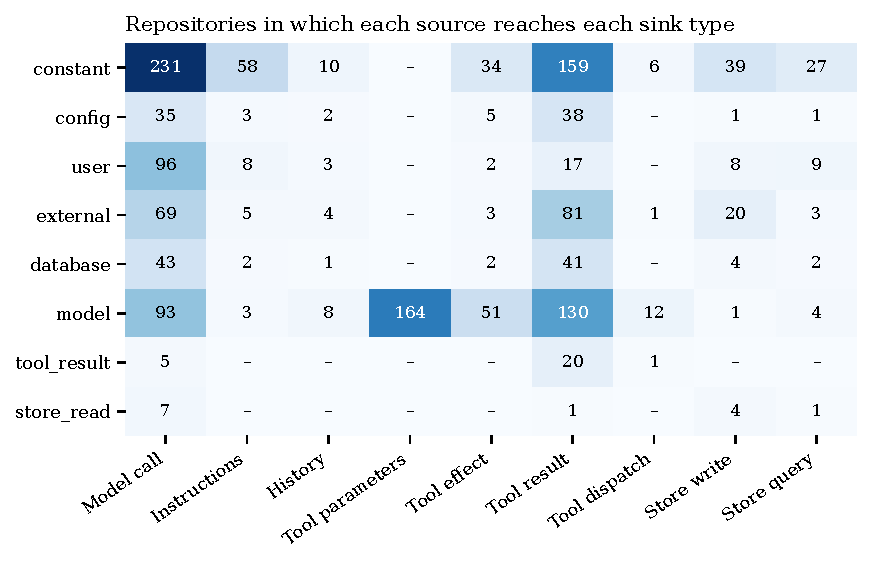
\includegraphics[width=0.9\linewidth]{Images/flow/source_to_sink.pdf}
  \caption{Number of applications in which each source class reaches each sink type (confirmed rules).}
  \label{fig:res-source-to-sink}
\end{figure}

\begin{table}[t]
\centering
\renewcommand{\arraystretch}{1.2}
\caption{Reach of each source class in AI-relevant code: occurrences that flow into at least one sink.}
\label{tab:res-reach}
\begin{tabular}{@{}lrrr@{}}
\toprule
\textbf{Source} & \textbf{Occurrences} & \textbf{Reaching a sink} & \textbf{Share} \\
\midrule
\texttt{config}      & 4{,}086 & 350 & 8.6\% \\
\texttt{user}        & 2{,}114 & 585 & 27.7\% \\
\texttt{external}    & 2{,}184 & 847 & 38.8\% \\
\texttt{database}    & 2{,}468 & 585 & 23.7\% \\
\texttt{model}       & 3{,}405 & 533 & 15.7\% \\
\texttt{store\_read} & 215     & 32  & 14.9\% \\
\bottomrule
\end{tabular}
\end{table}

\emph{Meaning:} configuration mostly selects models and endpoints and rarely becomes model input, while almost four in ten occurrences of external content and more than a quarter of the user input that appears in AI-relevant code end up in a sink.

% =============================================================================
\section{RQ3: How Prevalent Are the Preconditions for Attacks?}
\label{sec:res-rq3}

Table~\ref{tab:res-patterns} and Figure~\ref{fig:res-patterns} report the five risk patterns of Table~\ref{tab:df-patterns}.

\begin{table}[t]
\centering
\footnotesize
\renewcommand{\arraystretch}{1.25}
\setlength{\tabcolsep}{4pt}
\caption{Prevalence of the risk patterns. \emph{Confirmed}: precise rules; \emph{upper bound}: including heuristic detections.}
\label{tab:res-patterns}
\begin{tabular}{@{}>{\raggedright\arraybackslash}p{0.33\textwidth}>{\raggedright\arraybackslash}p{0.07\textwidth}>{\raggedright\arraybackslash}p{0.18\textwidth}>{\raggedright\arraybackslash}p{0.18\textwidth}>{\raggedright\arraybackslash}p{0.16\textwidth}@{}}
\toprule
\textbf{Pattern} & \textbf{V} & \textbf{Confirmed} & \textbf{Upper bound} & \textbf{Relative to} \\
\midrule
Untrusted content reaches a model call         & V1, V4 & 133/248 (53.6\%) & 140/256 (54.7\%) & apps with model calls \\
Indirect content reaches a model call          & V1     & 70/248 (28.2\%)  & 72/256 (28.1\%)  & apps with model calls \\
Untrusted or indirect content reaches instructions & V1, V4 & 34/256 (13.3\%) & 44/277 (15.9\%) & apps with model inputs \\
Tool returns outside content and a tool can execute or access files & V1, V3 & 27/165 (16.4\%) & 27/165 (16.4\%) & apps with tools \\
Untrusted store write whose content reaches a model & V6 & 3/59 (5.1\%) & 3/59 (5.1\%) & apps with stores \\
\bottomrule
\end{tabular}
\end{table}

% \begin{figure}[t]
%   \centering
%   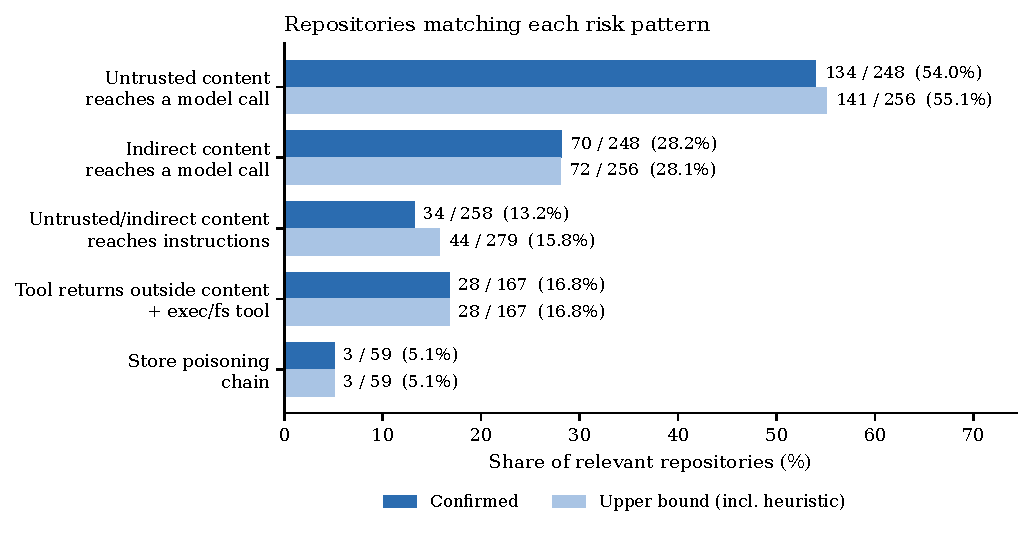
\includegraphics[width=0.85\linewidth]{Images/flow/risk_patterns.pdf}
%   \caption{Share of applications matching each risk pattern, relative to the applications in which it can occur.}
%   \label{fig:res-patterns}
% \end{figure}

\paragraph{Untrusted to model (V1, V4).} In 53.6\% of the applications that call a model, content controlled by a user or a third party reaches a model call. \emph{Meaning:} this is expected for conversational applications, and establishes that most applications are exposed to at least direct prompt injection.

\paragraph{Indirect to model (V1).} In 28.2\% of these applications, content that no user typed---web pages, retrieved documents, tool output---reaches a model call. \emph{Meaning:} in more than a quarter of the applications, an attacker who never interacts with the application can place instructions in front of its model.

\paragraph{Untrusted to instructions (V1, V4).} In 13.3\% of the applications with model inputs (15.9\% as upper bound), untrusted or indirect content reaches instructions or a system message. \emph{Meaning:} although instructions are mostly static, in these applications outside content receives the authority the model reserves for its developer. Listing~\ref{lst:case-instructions} shows a validated example: a chat route that takes its entire system prompt from the request body.

\noindent\begin{minipage}{\linewidth}
\begin{lstlisting}[language=JavaScript, caption={A chat route that takes its system prompt from the request body.}, label={lst:case-instructions}]
const { messages, systemPrompt, documentInputs } = await req.json();
let fullSystemPrompt = systemPrompt || "You are a helpful assistant.";
// ... documentInputs appended to fullSystemPrompt ...
const result = await generateText({ model, system: fullSystemPrompt, messages });
\end{lstlisting}
\end{minipage}

\paragraph{Tool risk combination (V1, V3).} In 16.4\% of the applications with tools, a tool returns outside content while a tool lets the model execute commands or access files. \emph{Meaning:} these applications contain both the entry point and the consequence of an indirect injection: content read by one tool can steer the model to misuse another (R6).

\paragraph{Store poisoning chain (V6).} Complete chains---untrusted content written to a store whose retrieved content reaches a model call---appear in 5.1\% of the applications with stores. \emph{Meaning:} this is a lower bound rather than evidence that memory poisoning is rare: almost half of these applications write untrusted content into a store, but the chain can only be observed when writes and reads are linked within the repository. The validation found an application that rebuilds its system prompt from persistent memories written by the model itself during the session, a complete persistent-injection loop whose memory content the analysis could not follow.

% =============================================================================
\section{RQ4: How Reliable Are the Measurements?}
\label{sec:res-rq4}

\paragraph{Recall.} On five repositories in which 21 model calls were identified by manual inspection, the confirmed rules find 12 (57\%), and 17 (81\%) including heuristic detections (Table~\ref{tab:res-recall}). The missed calls are made through agents kept in user-interface or framework state, which the analysis does not follow. Because these repositories also informed the rules for agent factories, the figures may be optimistic.

\begin{table}[t]
\centering
\renewcommand{\arraystretch}{1.2}
\caption{Recall of model-call detection on five manually inspected repositories (21 model calls).}
\label{tab:res-recall}
\begin{tabular}{@{}lrr@{}}
\toprule
\textbf{Detection} & \textbf{Found} & \textbf{Recall} \\
\midrule
Confirmed rules         & 12 & 57\% \\
Confirmed + heuristic   & 17 & 81\% \\
\bottomrule
\end{tabular}
\end{table}

\paragraph{Precision.} We judged 86 sink values sampled at random from 20 repositories not used during development (Table~\ref{tab:res-precision}). Of these, 76 are real inputs of a model, tool, or store, a sink precision of 88\%. Most false sinks come from a single large repository, where functions registered with a non-AI plugin and command system or sharing a generic name with a tool were mistaken for tools; the others are test files located next to the source code, which are now excluded from the results, and catch-all \texttt{**kwargs} parameters of tools. For the 76 real sinks, the reported sources were fully correct for 37 (49\%), partially correct for 27 (36\%)---the sources reported are right, but a kind of source is missing---and wrong for 12 (16\%). Values reported as static were always correct and values reported as dynamic were fully correct in 24 of 33 cases, whereas only 3 of the 33 values reported as undetermined had an origin that cannot be determined from the repository's code.\footnote{Including the two repositories used during development instead of their replacements gives a sink precision of 88\% (74 of 84) and fully correct sources for 54\% of the real sinks.}

\begin{table}[t]
\centering
\renewcommand{\arraystretch}{1.2}
\caption{Precision on 86 randomly sampled sink values from 20 repositories not used during development.}
\label{tab:res-precision}
\begin{tabular}{@{}lrr@{}}
\toprule
\textbf{Measure} & \textbf{Values} & \textbf{Share} \\
\midrule
\multicolumn{3}{@{}l}{\emph{Sinks}} \\
Real sinks, all detections         & 76 / 86 & 88\% \\
\quad confirmed rules              & 71 / 81 & 88\% \\
\quad heuristic                    & 5 / 5   & 100\% \\
\addlinespace[3pt]
\multicolumn{3}{@{}l}{\emph{Sources of the 76 real sinks}} \\
Fully correct                      & 37 & 49\% \\
Partially correct (a kind missing) & 27 & 36\% \\
Wrong                              & 12 & 16\% \\
\addlinespace[3pt]
\multicolumn{3}{@{}l}{\emph{Fully correct, by reported input class}} \\
Static                             & 10 / 10 & 100\% \\
Dynamic                            & 24 / 33 & 73\% \\
Undetermined                       & 3 / 33  & 9\% \\
\bottomrule
\end{tabular}
\end{table}

\emph{Meaning:} what the analysis reports as fixed or as set at run time can be relied on, and its errors are mostly omissions rather than false information: partially correct sources are incomplete, not wrong.

\paragraph{Completeness of traces.} A large share of inputs remains undetermined: 50.7\% of model-call inputs, 51.4\% of store writes, and 74.9\% of store queries (Table~\ref{tab:res-sinks}). This follows from the design of the analysis, which reports a value as undetermined instead of guessing its origin. The recorded reasons show where traces stop. For model calls, 37.4\% of the stopping points are parameters of functions without a caller in the repository, because they are invoked by a framework or messaging platform or reached through a provider or agent selected at run time; 30.5\% are calls into libraries or frameworks whose behaviour the analysis does not model, such as SDK clients, provider objects, and encoding functions; and 25.1\% are values built across more than five function boundaries. Tool results stop most often at unmodelled calls (50.4\%), reflecting that tools obtain their content from external services and libraries. Instructions stop mostly at parameters without a caller (42.6\%), since frameworks receive them from configuration and factory code, and 30.1\% of the stopping points of store reads are stores without a write in the repository, because stores are often filled by separate ingestion processes. The precision review confirms that these values are not unknowable: for 30 of the 33 undetermined values in the sample, a reader could establish the origin from the code, and it was predominantly user input, external content, or model output. Undetermined values therefore do not indicate that inputs are fixed or safe; the dynamic shares and risk-pattern counts are lower bounds.

\paragraph{Effect of the heuristic.} Heuristic detections change the applications with model calls little (248 to 256) but nearly double those with instructions (65 to 115), because instruction-like keyword arguments such as \texttt{prompt} are common in framework calls. \emph{Meaning:} the confirmed results are robust; the heuristic mainly affects instructions, whose upper bound should be read with care.

% =============================================================================
\section{Summary}
\label{sec:res-summary}

\begin{itemize}
  \item \textbf{RQ1.} The applications are dominated by direct use of vendor SDKs and MCP; 67.5\% pass data to a model, 43.5\% define tools, 15.6\% use a store, and 93 chain model calls.
  \item \textbf{RQ2.} Instructions are mostly fixed in the code (80.6\% static), while model calls, tools, and stores receive run-time data from users, third parties, and databases; external content enters above all through tools (80 applications).
  \item \textbf{RQ3.} Indirect content reaches a model in 28.2\% of the applications that call a model, untrusted content reaches instructions in 13.3\%, and 16.4\% of the applications with tools combine outside content with command or file access; complete memory-poisoning chains are observable in 5.1\% of the applications with stores, a lower bound.
  \item \textbf{RQ4.} Model-call detection reaches 57\% recall with confirmed rules and 81\% with the heuristic; 88\% of the reported sinks are real, and sources are fully correct for 49\% and at least partially correct for 84\% of them. Errors are mostly omissions, so the results are lower bounds.
\end{itemize}